\documentclass[12pt, letterpaper]{article}

% --- Packages ---
\usepackage[margin=1in]{geometry}
\usepackage{graphicx}
\usepackage{amsmath}
\usepackage{amssymb}
\usepackage{booktabs}
\usepackage{caption}
\usepackage{subcaption}
\usepackage{hyperref}
\usepackage{float}
\usepackage{siunitx}
\usepackage{enumitem}
\usepackage[numbers]{natbib}
\usepackage{fancyhdr}
\usepackage{setspace}

% --- Page style ---
\pagestyle{fancy}
\fancyhf{}
\rhead{ME 401 -- Project 2}
\lhead{Anaerobic Digestion \& Cogeneration}
\cfoot{\thepage}
\onehalfspacing

% --- Graphics path ---
\graphicspath{{./}{../output/}}

% --- Title ---
\title{%
  \textbf{Energy Recovery from Wastewater Sludge via Anaerobic Digestion and Steam Rankine Cogeneration} \\[0.5em]
  \large ME 401 Thermodynamics III -- Project 2 \\
  Boise State University
}
\author{Caleb H.}
\date{April 2026}

\begin{document}

\maketitle

\begin{abstract}
This report presents a coupled simulation of an anaerobic digester and a steam Rankine cogeneration plant for energy recovery from municipal wastewater sludge. The anaerobic digester is modeled as a continuous stirred-tank reactor operating at mesophilic conditions (\SI{35}{\celsius}), producing methane at a baseline rate of \SI{0.4}{\cubic\metre\per\cubic\metre\per\day}. The biogas fuels a regenerative Rankine cycle with steam extraction for process heating. At baseline conditions (reactor volume \SI{3000}{\cubic\metre}, serving a population of 100,000), the system produces \SI{104}{\kilo\watt} of net electrical output and \SI{166}{\kilo\watt} of process heat, achieving a combined heat and power efficiency of 54.2\% and offsetting 41.6\% of the plant's grid electricity demand. Parametric optimization reveals that a reactor volume of approximately \SI{7157}{\cubic\metre} is required for full electrical self-sufficiency. Economic analysis indicates a simple payback period of 2.9 years and annual avoidance of 365 tonnes of CO\textsubscript{2} emissions.
\end{abstract}

% ============================================================================
\section{Introduction}
% ============================================================================

Wastewater treatment is an energy-intensive process. Municipal treatment plants in the United States consume approximately \SI{0.3}{} to \SI{0.6}{\kilo\watt\hour\per\cubic\metre} of wastewater treated, representing a significant operational cost and carbon footprint \citep{nathia2018}. At the same time, the organic content of wastewater sludge represents a substantial, largely untapped energy resource. Anaerobic digestion (AD) converts this organic matter into biogas---a mixture of methane and carbon dioxide---through a series of biochemical reactions carried out by microbial communities in the absence of oxygen.

The biogas produced by AD can fuel combined heat and power (CHP) systems to simultaneously generate electricity and useful thermal energy, a configuration known as cogeneration. When the CHP system is integrated with the digester, the extracted process heat can maintain the reactor at its optimal operating temperature, creating a thermally self-sustaining loop. The electrical output can offset a portion---or potentially all---of the treatment plant's grid electricity consumption.

This project models and evaluates such an integrated system. The objectives are threefold:
\begin{enumerate}[noitemsep]
  \item Develop a coupled steady-state simulation of an anaerobic digester and a steam Rankine cogeneration plant.
  \item Perform parametric analysis and numerical optimization to characterize system performance across a range of operating conditions.
  \item Compare the CHP-integrated system to conventional grid-powered operation in terms of energy, cost, and emissions.
\end{enumerate}

The simulation is implemented in Python, using CoolProp for thermodynamic property evaluation and SciPy for numerical optimization. All source code, unit tests, and generated data accompany this report.

% ============================================================================
\section{Methodology}
% ============================================================================

\subsection{System Overview}

The modeled system consists of two coupled subsystems (Figure~\ref{fig:system_diagram}):
\begin{enumerate}[noitemsep]
  \item \textbf{Anaerobic Digester}: A continuous stirred-tank reactor (CSTR) that receives wastewater sludge and produces biogas through mesophilic anaerobic digestion.
  \item \textbf{Cogeneration Plant}: A steam Rankine cycle with extraction that converts biogas thermal energy into electricity and process heat.
\end{enumerate}

The two subsystems are coupled: biogas from the digester provides fuel for the CHP boiler, and extracted steam from the turbine provides process heat to maintain digester temperature. The extraction fraction is determined iteratively to match the digester's thermal demand.

\begin{figure}[H]
  \centering
  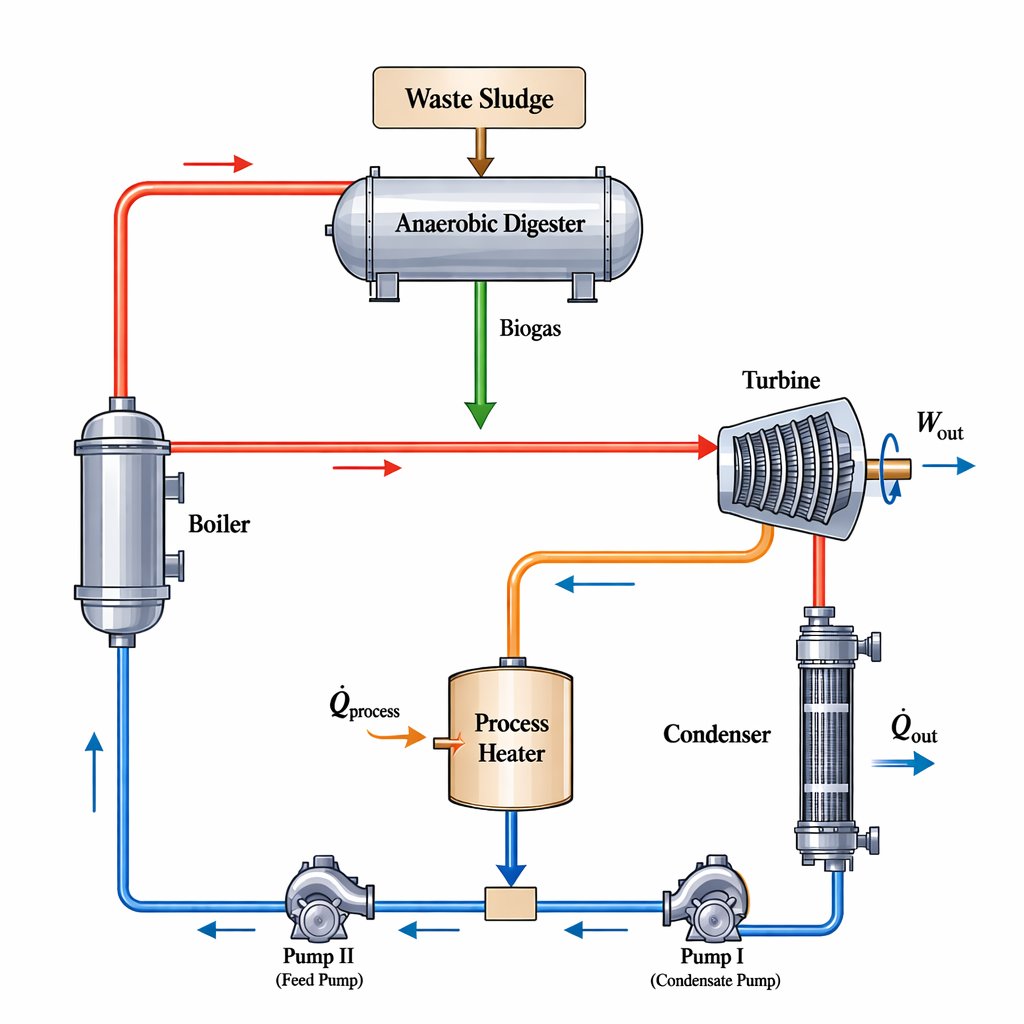
\includegraphics[width=0.9\textwidth]{System_flow_diagram.png}
  \caption{Schematic of the coupled anaerobic digester and cogeneration system. Biogas flows from the digester to the CHP plant; process heat returns to maintain digester temperature.}
  \label{fig:system_diagram}
\end{figure}

\subsection{Anaerobic Digester Model}

The digester is modeled as a steady-state CSTR operating under mesophilic conditions. The key governing equations are drawn from the literature \citep{nathia2018}.

\paragraph{Hydraulic Retention Time (HRT).}
The HRT characterizes the average residence time of sludge in the reactor:
\begin{equation}
  \text{HRT} = \frac{V}{Q}
  \label{eq:hrt}
\end{equation}
where $V$ is the reactor volume (\si{\cubic\metre}) and $Q$ is the volumetric feed rate (\si{\cubic\metre\per\day}). For mesophilic digesters, typical HRT values range from 10 to 40 days \citep{nathia2018}. A baseline value of 20 days is used throughout this analysis.

\paragraph{Organic Loading Rate (OLR).}
The OLR quantifies the mass of volatile solids fed per unit reactor volume per day:
\begin{equation}
  \text{OLR} = \frac{Q \cdot \text{VS}_\text{in}}{V}
  \label{eq:olr}
\end{equation}
where $\text{VS}_\text{in}$ is the influent volatile solids concentration (\si{\kilo\gram\per\cubic\metre}).

\paragraph{Methane Production.}
The volumetric methane production rate (VMP) is taken as \SI{0.4}{\cubic\metre} CH\textsubscript{4} per \si{\cubic\metre} of reactor volume per day, consistent with values reported for optimized sewage sludge digestion. The total methane production is:
\begin{equation}
  \dot{V}_{\text{CH}_4} = \text{VMP} \times V
  \label{eq:ch4}
\end{equation}

Biogas composition is assumed to be 60\% CH\textsubscript{4} and 40\% CO\textsubscript{2} by volume, within the 55--70\% methane range reported in the literature \citep{nathia2018}. The thermal energy content of the biogas is:
\begin{equation}
  \dot{Q}_\text{biogas} = \dot{V}_{\text{CH}_4} \times \text{LHV}_{\text{CH}_4}
  \label{eq:q_biogas}
\end{equation}
where $\text{LHV}_{\text{CH}_4} = \SI{35.8}{\mega\joule\per\cubic\metre}$ at standard conditions.

\paragraph{Digester Heat Demand.}
The digester requires thermal input for two purposes:
\begin{enumerate}[noitemsep]
  \item \textit{Sludge heating}: Raising incoming sludge from ambient to operating temperature:
  \begin{equation}
    \dot{Q}_\text{sludge} = \dot{m} \cdot c_p \cdot (T_\text{op} - T_\text{feed})
    \label{eq:q_sludge}
  \end{equation}
  where $\dot{m}$ is the sludge mass flow rate, $c_p \approx \SI{4.18}{\kilo\joule\per\kilo\gram\per\kelvin}$, $T_\text{op} = \SI{35}{\celsius}$, and $T_\text{feed} = \SI{15}{\celsius}$.

  \item \textit{Wall heat losses}: Conduction through the insulated reactor shell:
  \begin{equation}
    \dot{Q}_\text{loss} = U \cdot A \cdot (T_\text{op} - T_\text{amb})
    \label{eq:q_loss}
  \end{equation}
  where $U = \SI{1.0}{\watt\per\square\metre\per\kelvin}$ for an insulated concrete digester, and $A$ is the outer surface area of the cylindrical vessel.
\end{enumerate}

\subsection{Cogeneration Plant Model}

The CHP system is modeled as a regenerative Rankine cycle with steam extraction for process heating. The working fluid is water; all thermodynamic properties are evaluated using CoolProp \citep{coolprop}.

\paragraph{Cycle Configuration.}
The cycle comprises eight state points and six components:
\begin{itemize}[noitemsep]
  \item \textbf{State 1}: Condenser exit (saturated liquid, $P_\text{cond} = \SI{10}{\kilo\pascal}$)
  \item \textbf{State 2}: Pump~I exit (compressed liquid, $P_\text{extract} = \SI{500}{\kilo\pascal}$)
  \item \textbf{State 3}: Process heater exit (saturated liquid, $P_\text{extract}$)
  \item \textbf{State 4}: Mixing chamber exit (liquid, $P_\text{extract}$)
  \item \textbf{State 5}: Pump~II exit (compressed liquid, $P_\text{boiler} = \SI{6}{\mega\pascal}$)
  \item \textbf{State 6}: Boiler exit (superheated steam, $P_\text{boiler}$, $T = \SI{450}{\celsius}$)
  \item \textbf{State 7}: Turbine extraction (steam, $P_\text{extract}$)
  \item \textbf{State 8}: Turbine exhaust (wet steam, $P_\text{cond}$)
\end{itemize}

\paragraph{Energy Balance Equations.}
For a total steam mass flow rate $\dot{m}$ and extraction fraction $y$ (fraction of steam diverted to the process heater), the component energy balances per unit mass of total steam flow are:

\textit{Turbine} (with isentropic efficiency $\eta_t = 0.85$):
\begin{equation}
  w_t = (h_6 - h_7) + (1-y)(h_7 - h_8)
  \label{eq:w_turbine}
\end{equation}

\textit{Pumps} (with isentropic efficiency $\eta_p = 0.80$):
\begin{equation}
  w_{p1} = (1-y)(h_2 - h_1), \quad w_{p2} = h_5 - h_4
  \label{eq:w_pumps}
\end{equation}

\textit{Boiler} (with thermal efficiency $\eta_b = 0.85$):
\begin{equation}
  q_\text{in} = h_6 - h_5, \quad \dot{m} = \frac{\dot{Q}_\text{biogas} \cdot \eta_b}{q_\text{in}}
  \label{eq:q_boiler}
\end{equation}

\textit{Process heater}:
\begin{equation}
  q_\text{process} = y(h_7 - h_3)
  \label{eq:q_process}
\end{equation}

\textit{Mixing chamber} (adiabatic):
\begin{equation}
  h_4 = (1-y) \cdot h_2 + y \cdot h_3
  \label{eq:mixing}
\end{equation}

The extraction fraction $y$ is determined iteratively by requiring the process heat delivered to equal the digester thermal demand:
\begin{equation}
  y = \frac{\dot{Q}_\text{digester}}{\dot{m} \cdot (h_7 - h_3)}
  \label{eq:y}
\end{equation}

Since $\dot{m}$ depends on $h_5$, which depends on $h_4$, which depends on $y$, the system is solved iteratively until convergence.

\paragraph{Performance Metrics.}
\begin{align}
  \eta_\text{elec} &= \frac{\dot{W}_\text{net,elec}}{\dot{Q}_\text{fuel}} \label{eq:eta_elec} \\
  \eta_\text{thermal} &= \frac{\dot{Q}_\text{process}}{\dot{Q}_\text{fuel}} \label{eq:eta_thermal} \\
  \eta_\text{CHP} &= \frac{\dot{W}_\text{net,elec} + \dot{Q}_\text{process}}{\dot{Q}_\text{fuel}} \label{eq:eta_chp}
\end{align}

\subsection{Numerical Optimization}

Three optimization problems are solved using SciPy:
\begin{enumerate}[noitemsep]
  \item \textbf{Self-sufficiency}: Minimize reactor volume subject to $\dot{W}_\text{net} \geq \dot{W}_\text{WWTP}$, using bounded scalar optimization.
  \item \textbf{Maximum power}: Optimize boiler pressure, superheat temperature, and extraction pressure to maximize $\dot{W}_\text{net}$ at fixed reactor volume, using differential evolution.
  \item \textbf{Maximum CHP efficiency}: Same decision variables, maximizing $\eta_\text{CHP}$.
\end{enumerate}

\subsection{Grid Comparison Assumptions}

The CHP system is compared against a conventional grid-powered plant using the following assumptions:
\begin{itemize}[noitemsep]
  \item Grid electricity cost: \$0.10/kWh
  \item Grid carbon intensity: \SI{0.40}{\kilo\gram}~CO\textsubscript{2}/kWh
  \item WWTP specific energy: \SI{0.40}{\kilo\watt\hour\per\cubic\metre} wastewater
  \item CHP capital cost: \$2500/kW installed
\end{itemize}

% ============================================================================
\section{Results}
% ============================================================================

\subsection{Baseline Performance}

Table~\ref{tab:baseline} summarizes the baseline simulation results for a \SI{3000}{\cubic\metre} reactor serving a population of 100,000.

\begin{table}[H]
  \centering
  \caption{Baseline simulation results (V = \SI{3000}{\cubic\metre}, population = 100,000).}
  \label{tab:baseline}
  \begin{tabular}{@{}lrl@{}}
    \toprule
    \textbf{Parameter} & \textbf{Value} & \textbf{Unit} \\
    \midrule
    \multicolumn{3}{l}{\textit{Digester}} \\
    Hydraulic retention time & 20.0 & days \\
    Organic loading rate & 1.25 & kg VS/(m\textsuperscript{3}$\cdot$day) \\
    Methane production & 1200 & m\textsuperscript{3}/day \\
    Biogas energy content & 497 & kW \\
    Digester heat demand & 166 & kW \\
    \midrule
    \multicolumn{3}{l}{\textit{Cogeneration Plant}} \\
    Steam mass flow & 0.147 & kg/s \\
    Extraction fraction ($y$) & 0.522 & -- \\
    Net electrical output & 104 & kW \\
    Process heat delivered & 166 & kW \\
    Condenser heat rejected & 148 & kW \\
    Electrical efficiency & 20.9 & \% \\
    CHP efficiency & 54.2 & \% \\
    \midrule
    \multicolumn{3}{l}{\textit{Grid Impact}} \\
    WWTP electricity demand & 250 & kW \\
    Grid offset & 41.6 & \% \\
    \bottomrule
  \end{tabular}
\end{table}

The thermodynamic state points for the Rankine cycle are presented in Table~\ref{tab:states}.

\begin{table}[H]
  \centering
  \caption{Thermodynamic state points for the baseline Rankine cycle.}
  \label{tab:states}
  \begin{tabular}{@{}clrrrrr@{}}
    \toprule
    \textbf{State} & \textbf{Location} & \textbf{$P$ (kPa)} & \textbf{$T$ (\si{\celsius})} & \textbf{$h$ (kJ/kg)} & \textbf{$s$ (kJ/kg$\cdot$K)} & \textbf{$x$} \\
    \midrule
    1 & Condenser exit       &    10 &  45.8 &  192 & 0.649 & 0.000 \\
    2 & Pump I exit          &   500 &  45.9 &  192 & 0.650 & -- \\
    3 & Process heater exit  &   500 & 151.8 &  640 & 1.860 & 0.000 \\
    4 & Mixing chamber exit  &   500 & 101.5 &  426 & 1.324 & -- \\
    5 & Pump II exit         &  6000 & 102.3 &  433 & 1.328 & -- \\
    6 & Boiler exit          &  6000 & 450.0 & 3303 & 6.722 & -- \\
    7 & Turbine extraction   &   500 & 172.4 & 2796 & 6.930 & -- \\
    8 & Turbine exhaust      &    10 &  45.8 & 2285 & 7.212 & 0.875 \\
    \bottomrule
  \end{tabular}
\end{table}

At state 8 (turbine exhaust), the steam quality of 0.875 confirms that the flow remains within acceptable wet-steam limits for turbine operation. The high extraction fraction ($y = 0.522$) reflects the substantial thermal demand of heating incoming sludge from \SI{15}{\celsius} to \SI{35}{\celsius}.

\subsection{Parametric Analysis}

\subsubsection{Reactor Volume}

Figure~\ref{fig:volume} shows how net electrical output and CHP efficiency vary with reactor volume at constant HRT (20 days). The relationship is approximately linear because methane production scales directly with volume, while the extraction fraction decreases slightly at larger scales due to sub-linear growth in wall heat losses. The WWTP demand of \SI{250}{\kilo\watt} is met at a reactor volume of approximately \SI{7000}{\cubic\metre}.

\begin{figure}[H]
  \centering
  \includegraphics[width=0.85\textwidth]{fig1_volume_sweep.pdf}
  \caption{Net electrical output and CHP efficiency as a function of reactor volume. The dashed red line indicates the WWTP electricity demand (\SI{250}{\kilo\watt}) for a plant serving 100,000 people.}
  \label{fig:volume}
\end{figure}

\subsubsection{Boiler Pressure}

Figure~\ref{fig:boiler} presents the effect of boiler pressure on CHP performance at fixed digester conditions. Both net electrical output and electrical efficiency increase with boiler pressure, as higher pressure ratios across the turbine produce more work per unit mass of steam. However, the gains exhibit diminishing returns above approximately \SI{8}{\mega\pascal}, consistent with fundamental Rankine cycle behavior.

\begin{figure}[H]
  \centering
  \includegraphics[width=0.85\textwidth]{fig2_boiler_pressure.pdf}
  \caption{Effect of boiler pressure on net electrical output and electrical efficiency.}
  \label{fig:boiler}
\end{figure}

\subsubsection{Extraction Pressure}

Figure~\ref{fig:extraction} illustrates the trade-off inherent in extraction pressure selection. At lower extraction pressures, more work is extracted in the high-pressure turbine stage before the bleed point, and the extraction steam carries more enthalpy, so a smaller fraction $y$ suffices to meet the digester heat demand. This results in higher electrical output at lower extraction pressures but a modest decrease in overall CHP efficiency, as more energy is rejected in the condenser.

\begin{figure}[H]
  \centering
  \includegraphics[width=\textwidth]{fig3_extraction_pressure.pdf}
  \caption{Effect of extraction pressure on (a) power and heat output, and (b) system efficiencies.}
  \label{fig:extraction}
\end{figure}

\subsection{Energy Balance}

Figure~\ref{fig:energy} presents the energy flow through the system at baseline conditions. Of the \SI{497}{\kilo\watt} of biogas input, approximately 85\% is transferred to the steam cycle via the boiler. Electrical output and useful process heat account for the majority of that energy, with condenser losses making up the remainder.

\begin{figure}[H]
  \centering
  \includegraphics[width=0.85\textwidth]{fig4_energy_balance.pdf}
  \caption{Energy balance for the baseline system, showing the flow from biogas input to useful outputs and losses.}
  \label{fig:energy}
\end{figure}

\subsection{Grid Comparison}

Figure~\ref{fig:grid} compares the CHP-integrated plant to grid-only operation on an annual basis. The CHP system offsets 42\% of grid electricity demand, saving approximately \$91,000 per year and avoiding 365 tonnes of CO\textsubscript{2} emissions annually.

\begin{figure}[H]
  \centering
  \includegraphics[width=\textwidth]{fig5_grid_comparison.pdf}
  \caption{Annual comparison of CHP-integrated vs.\ grid-only operation: (a) electricity source, (b) cost, (c) CO\textsubscript{2} emissions.}
  \label{fig:grid}
\end{figure}

\subsection{Optimization Results}

Table~\ref{tab:optimization} summarizes the three optimization runs.

\begin{table}[H]
  \centering
  \caption{Optimization results for three objective functions.}
  \label{tab:optimization}
  \begin{tabular}{@{}lccc@{}}
    \toprule
    & \textbf{Self-Sufficiency} & \textbf{Max Power} & \textbf{Max CHP Eff.} \\
    \midrule
    Reactor volume (m\textsuperscript{3}) & 7157 & 3000 (fixed) & 3000 (fixed) \\
    $P_\text{boiler}$ (MPa) & 6.0 (fixed) & 12.0 & 12.0 \\
    $T_\text{superheat}$ (\si{\celsius}) & 450 (fixed) & 550 & 550 \\
    $P_\text{extract}$ (kPa) & 500 (fixed) & 200 & 200 \\
    $\dot{W}_\text{net}$ (kW) & 250.0 & 125.1 & 125.1 \\
    $\eta_\text{elec}$ (\%) & 20.9 & 25.2 & 25.2 \\
    $\eta_\text{CHP}$ (\%) & 54.2 & 58.5 & 58.5 \\
    \bottomrule
  \end{tabular}
\end{table}

As shown in Table~\ref{tab:optimization}, the self-sufficiency optimization requires a reactor volume approximately 2.4 times the baseline. The maximum-power and maximum-efficiency optimizations converge to the same operating point, yielding a 20\% improvement in electrical output over baseline.

\subsection{Breakeven Analysis}

Figure~\ref{fig:breakeven} shows the required reactor volume for electrical self-sufficiency as a function of population served. The relationship is approximately linear, providing a practical design reference for plants at various scales.

\begin{figure}[H]
  \centering
  \includegraphics[width=0.85\textwidth]{fig6_breakeven_population.pdf}
  \caption{Breakeven reactor volume (for electrical self-sufficiency) as a function of population served.}
  \label{fig:breakeven}
\end{figure}

\subsection{Efficiency Across Scales}

Table~\ref{tab:efficiency} presents system performance at four reactor scales. Electrical efficiency is nearly constant (20.7--21.1\%), while CHP efficiency decreases slightly at larger scales because wall heat losses grow sub-linearly with volume, reducing the extraction fraction.

\begin{table}[H]
  \centering
  \caption{System performance at various reactor scales (constant HRT = 20 days).}
  \label{tab:efficiency}
  \begin{tabular}{@{}lrrrrrr@{}}
    \toprule
    \textbf{Scale} & \textbf{$V$ (m\textsuperscript{3})} & \textbf{CH\textsubscript{4} (m\textsuperscript{3}/d)} & \textbf{$\dot{W}_\text{elec}$ (kW)} & \textbf{$\dot{Q}_\text{proc}$ (kW)} & \textbf{$\eta_\text{elec}$ (\%)} & \textbf{$\eta_\text{CHP}$ (\%)} \\
    \midrule
    Small      & 1000  &  400 &  34 &  58 & 20.7 & 55.6 \\
    Medium     & 3000  & 1200 & 104 & 166 & 20.9 & 54.2 \\
    Large      & 6000  & 2400 & 209 & 324 & 21.1 & 53.6 \\
    Very Large & 10000 & 4000 & 350 & 533 & 21.1 & 53.3 \\
    \bottomrule
  \end{tabular}
\end{table}

% ============================================================================
\section{Discussion}
% ============================================================================

\subsection{Thermodynamic Trade-offs}

The central trade-off in this CHP system is between electrical output and process heat delivery, mediated by the extraction fraction $y$. At baseline, over half of the steam (52.2\%) is extracted for digester heating, significantly reducing turbine power output. This is driven primarily by the sludge heating load (\SI{148}{\kilo\watt} of the total \SI{166}{\kilo\watt} demand), which is proportional to the temperature difference between feed and operating conditions.

Several strategies could reduce this thermal penalty:
\begin{itemize}[noitemsep]
  \item \textit{Sludge preheating} using waste heat from the condenser or digestate
  \item \textit{Heat recovery} from the hot digestate stream via a counter-current heat exchanger
  \item \textit{Improved insulation} to reduce wall losses (though these are already modest)
\end{itemize}

Implementing a sludge-digestate heat exchanger could recover a substantial fraction of the sludge heating load, meaningfully reducing $y$ and increasing electrical output.

\subsection{Boiler Pressure and Superheat}

The optimization results indicate that operating at higher boiler pressure (\SI{12}{\mega\pascal}) and superheat temperature (\SI{550}{\celsius}) improves both electrical output and CHP efficiency. This is expected from Rankine cycle theory: higher mean temperature of heat addition improves Carnot-limited efficiency. However, these conditions require more expensive metallurgy and increase equipment cost. For a biogas-fired system of this scale, the baseline conditions (\SI{6}{\mega\pascal}, \SI{450}{\celsius}) represent a practical compromise between thermodynamic performance and capital cost.

\subsection{Self-Sufficiency Feasibility}

The self-sufficiency analysis reveals that a reactor volume roughly 2.4 times the baseline (\SI{7157}{\cubic\metre} vs.\ \SI{3000}{\cubic\metre}) is needed for electrical independence. This corresponds to a treatment plant serving approximately 240,000 people---a large but not unusual municipal system. Smaller plants can still benefit significantly from partial grid offset: even the baseline configuration reduces grid purchases by 42\%.

\subsection{Economic Viability}

The estimated simple payback of 2.9 years is attractive by infrastructure investment standards, where paybacks under 5 years are generally considered favorable. This estimate is conservative in that it does not account for:
\begin{itemize}[noitemsep]
  \item Revenue from renewable energy credits or carbon credits
  \item Avoided sludge disposal costs (the digestate has value as fertilizer)
  \item Escalation of grid electricity prices over the 20+ year equipment lifetime
  \item Potential revenue from excess electricity sold back to the grid (at self-sufficient scale)
\end{itemize}

\subsection{Limitations and Assumptions}

Several simplifying assumptions should be noted:
\begin{enumerate}[noitemsep]
  \item \textbf{Steady-state model}: Real digesters exhibit transient behavior during startup and in response to feed variability. A time-resolved model would capture these dynamics but is beyond the scope of this analysis.
  \item \textbf{Fixed methane yield}: The VMP of \SI{0.4}{\cubic\metre\per\cubic\metre\per\day} is treated as constant. In practice, yield depends on sludge composition, OLR, and microbial community health.
  \item \textbf{Ideal mixing}: The CSTR assumption implies perfect mixing, which may overestimate performance relative to real reactors with dead zones.
  \item \textbf{No parasitic loads}: Digester mixing energy, pumping, and other auxiliary loads are not subtracted from the net electrical output.
  \item \textbf{Simple economic model}: The payback calculation uses constant energy prices and does not include maintenance costs, financing, or time value of money.
\end{enumerate}

\subsection{Comparison to Literature}

The biogas energy yield of \SI{0.7}{} to \SI{2.0}{\kilo\watt\hour\per\cubic\metre} of biogas reported by Cheng and Wang (2013), as cited in N\'{a}thia-Neves et al.~\citep{nathia2018}, corresponds to our computed value of approximately \SI{6.0}{\kilo\watt\hour\per\cubic\metre} of methane (or \SI{3.6}{\kilo\watt\hour\per\cubic\metre} of biogas at 60\% CH\textsubscript{4}), which falls within the upper range. Our CHP electrical efficiency of 20.9\% is consistent with typical small-scale steam Rankine systems, which generally achieve 15--30\% electrical efficiency depending on scale and operating conditions.

% ============================================================================
\section{Conclusion}
% ============================================================================

This analysis demonstrates that integrating anaerobic digestion with steam Rankine cogeneration is a thermodynamically sound and economically viable strategy for energy recovery at municipal wastewater treatment plants. The key conclusions are:

\begin{enumerate}
  \item At baseline conditions (3,000~m\textsuperscript{3} reactor, 100,000 population), the CHP system produces \SI{104}{\kilo\watt} of net electrical output at 20.9\% electrical efficiency and 54.2\% overall CHP efficiency, offsetting 42\% of the plant's grid electricity demand.

  \item Full electrical self-sufficiency requires a reactor volume of approximately \SI{7,157}{\cubic\metre}---achievable for plants serving 200,000+ people.

  \item The system achieves a simple payback period of 2.9 years and avoids 365 tonnes of CO\textsubscript{2} emissions annually at the baseline scale.

  \item Optimizing CHP parameters (higher boiler pressure and superheat, lower extraction pressure) can improve electrical output by approximately 20\%, though at higher capital cost.
\end{enumerate}

\textbf{Recommendation}: For municipal treatment plants serving populations above 50,000, CHP integration with anaerobic digestion is recommended as a cost-effective upgrade that improves energy independence, reduces operating costs, and lowers carbon emissions. Plants should prioritize sludge-digestate heat recovery to minimize the extraction fraction and maximize electrical output. For smaller plants, the economic case depends on local electricity prices and available incentives.

% ============================================================================
% References
% ============================================================================
\begin{thebibliography}{9}

\bibitem{nathia2018}
G.~N\'{a}thia-Neves, M.~Berni, G.~Dragone, S.~I.~Mussatto, and T.~Forster-Carneiro,
``Anaerobic digestion process: technological aspects and recent developments,''
\textit{Int. J. Environ. Sci. Technol.}, vol.~15, pp.~2033--2046, 2018.
\newblock \href{https://doi.org/10.1007/s13762-018-1682-2}{doi:10.1007/s13762-018-1682-2}.

\bibitem{coolprop}
I.~H.~Bell, J.~Wronski, S.~Quoilin, and V.~Lemort,
``Pure and pseudo-pure fluid thermophysical property evaluation and the open-source thermophysical property library CoolProp,''
\textit{Ind. Eng. Chem. Res.}, vol.~53, no.~6, pp.~2498--2508, 2014.

\bibitem{cengel}
Y.~A.~\c{C}engel and M.~A.~Boles,
\textit{Thermodynamics: An Engineering Approach}, 8th ed.
McGraw-Hill, 2015.

\bibitem{kothari2014}
R.~Kothari, A.~K.~Pandey, S.~Kumar, V.~V.~Tyagi, and S.~K.~Tyagi,
``Different aspects of dry anaerobic digestion for bio-energy: An overview,''
\textit{Renew. Sustain. Energy Rev.}, vol.~39, pp.~174--195, 2014.

\bibitem{appels2008}
L.~Appels, J.~Baeyens, J.~Degr\`{e}ve, and R.~Dewil,
``Principles and potential of the anaerobic digestion of waste-activated sludge,''
\textit{Prog. Energy Combust. Sci.}, vol.~34, pp.~755--781, 2008.

\end{thebibliography}

\end{document}
